\documentclass{article}
\usepackage[utf8]{inputenc}
\usepackage{graphicx}
\usepackage[a4paper, total={8in, 10.5in}]{geometry}
\usepackage{rotating}
\usepackage{afterpage}
\usepackage{url}

\usepackage{algorithm}
\usepackage{algpseudocode}

\usepackage{amsmath}

\usepackage{mathtools}
\usepackage{tabularx}

\usepackage{caption}
\usepackage{subcaption}

\title{Seismic Moment Tensor Inversion}
\author{Maximilian Williams}
\date{November 2021}

\begin{document}

\maketitle


\section*{What is this?}
This document is a brief explanation detailing my thinking for a small program I wrote to invert seismogram data for the seismic moment tensor of the source.

\section*{The goal}
The goal of the program is to invert for the seismic moment tensor given synthetic seismogram data, precomputed Green's functions and the locations of the stations. 

\section*{Assumptions}

\begin{itemize}
  \item The seismograms are cleaned, so they have average of zero, band pass filters were already applied etc...
\end{itemize}


\section*{Conventions}
The seismic moment tensor will always be formmated in cartesian coordaintes. 
\newline
The greens functions and seismograms will have vertical (Z), radial (R) and transverse (T) directions.

\section*{Explanation}
We have siesmograms each with three components, $d_Z(p,t)$ vertical (Z), $d_R(p,t)$ radial (R) and $d_T(p, t)$ transverse (T). Here $p$ is the location of the station which is at azimuthal angle $\theta_p$ from the event. We model the source as a set of force couples whose configuration is encoded in the seismic moment tensor $M$. The synthetic seismograms are then given by:
\begin{equation}
	\begin{split}
	d'_Z(p,t) = M_{xx} (ZSS/2 *\cos{2 \theta_p} - ZDD/6 + ZEP/3)
	\\
	+ M_{yy} (-ZSS/2 *\cos{2 \theta_p} - ZDD/6 + ZEP/3) \\
	+ M_{zz} (ZDD/3 + ZEP/3) \\ 
	+ M_{xy} (ZSS \sin{2 \theta_p}) \\ 
	+ M_{xz} (ZDS \cos{\theta_p}) \\ 
	+ M_{yz} (ZDS \sin{\theta_p})
	\end{split}
\end{equation}
\begin{equation}
	\begin{split}
	d'_R(p,t) = M_{xx} (RSS/2 * \cos{2 \theta_p} - RDD/6 + REP/3) \\
	+ M_{yy} (-RSS/2 * \cos{2 \theta_p} - RDD/6 + REP/3  ) \\
	+ M_{zz} (RDD/3 + REP/3) \\
	+ M_{xy} (RSS\sin{2 \theta_p})\\
	+ M_{xz} (RDS \cos{\theta_p}) \\
	+ M_{yz} (RDS \sin{\theta_p})
	\end{split}
\end{equation}

\begin{equation}
	\begin{split}
	d'_T(p,t) = M_{xx} (TSS/2 * \sin{2 \theta_p}) \\
	+ M_{yy} (-TSS/2 * \sin{2 \theta_p}  ) \\
	+ M_{xy} (-TTS \cos{2 \theta_p} \\
	+ M_{xz} (TDS \sin{\theta_p}) \\
	+ M_{yz} (-TDS \cos{\theta_p})
	\end{split}
\end{equation}
Here SS is the vertical strike-slip, DD the $\frac{\pi}{4}$ dip slip, DS the vertical dip-slip and EP the explosive component of the Green's functions with Z, T and R being the vertical, transverse and radial components. This method of computing the synthetic seismograms is from lecture 2 week 5 of PHYS3070.
\newline
The computation of the synthetic data $d'_{n}(p,t)$ $n\in{Z,R,T}$ is the forwards problem. We will call obtaining the $M$ such that $d$ and $d'$ are the most similar the inverse problem.

\section*{Program Inputs}
The main program is main.py. It can be run using "python3 main.py". 
\newline
The program takes two types of files to run. The first set of files are to be located in a folder called "Greensfunctions". Within the folder 
"Greensfunctions" are located greens functions in .sac format. The files are named XX.XXXX.00.DD.0000.YYY. Here X entries indicate the station, Ds 
indicate the depth and Ys indicate the component of the greens functions. For example, BK.FARB.00.5.0000.REX is the greens function between the event at a 
depth of 5 km and the station BK.FARB with component REX (radial explosive). The other file input is naming and location information about the stations 
that we will use to do the inversion. This is called "stationInformation.csv". This csv file contains two columns. The first column contains the names of 
the station used for the inversion. The second column contains the azimuthal angle the station is at relative to the event location. Finally, a depth for 
the source is specified manually in the program. By default it is 5km.

\section*{Method}
The program does not take real seismograms, but we still want to show that it can invert for the moment tensor. To do this we arbitrarily define a target moment tensor $M_t$. We then perform the forwards problem to obtain the target data $d_t$. We now treat $d_t$ as real data and try to find the moment tensor associated with it which is ofcourse ideally $M_t$. 
\newline
I have chosen to view the inverse problem as an optimization problem. Specifically, I see the inverse problem as optimizing $M$ such that it maximises 
$g(d',d_t)$ where $g(\cdot, \cdot)$ is the score metric defined in the appendix. Ideally, this returns $M$ close to $M_t$. We note that we tend not to have large numbers
 of stations and the seismograms tend not to be very long. Therefore, we can expect computation of the forwards problem to be very fast on modern 
 computers. For this reason, I chose to use a genetic algorithm to optimize $M$.

\subsection*{Genetic Algorithms}
Genetic algorithms are a broad class of algorithms which use methods inspired by natural evolution to optimize. Here I used a basic variant. The algorithm generates a random 
population of seismic moment tensors. (1) For each seismic moment tensor in the population, the forwards problem is computed and the score computed (defined in appendix). The highest scoring
seismic moment tensors are then bred together to produce a new population \footnote{When we breed the population, we pick two moment tensors and average them. The selection of individuals is done probabilistically, with the probability of being picked to breed being proportional to the score. This breeding process is repeated over and over until we generate a new population.} (2). (1) to (2) is then repeated $epochs$ number of times. Once complete, the average seismic moment tensor from the last 
population is returned. This algorithm is detailed below. 
\begin{algorithm}[h!]
\caption{}\label{alg:TLBM}
\begin{algorithmic}

\State $Ms \gets \{\}$
\State $S \gets \{\}$
\State epoch $\gets 0$

\State $Ms \gets generateRandomPopulation(populationSize)$
\While{epoch $<$ epochs}
	\State $S \gets scorePopulation(Ms)$
	\State $Ms \gets breedPopulation(Ms, S)$
	\State epoch $\gets$ epoch $+1$
\EndWhile
\newline
\Return{average(Ms)}
\end{algorithmic}
\end{algorithm}

\section*{Results}
%% Here I will have a result were I invert for a simple double couple mechanism
%% I will show the resulting moment tensor and the siemsograms from the inversion
%% this will show that my program works

%% I will then add some random noise and perform the test again


I tested three inversions in my code. A DC mechanism, explosive and CLVD mechanism.
\subsection*{DC results}
The target moment tensor is:
\begin{gather}
	\begin{pmatrix}
	0 & 0.5 & 0 \\
	0.5 & 0 & 0 \\
	0 & 0 & 0 
	\end{pmatrix}
\end{gather}
The program inverts the moment tensor and finds it to be:
\begin{gather}
	\begin{pmatrix}
	-0.07 & 0.48 & -0.00 \\
	0.48 & 0.04 & 0.00 \\
	-0.00 & 0.00 & -0.04 
	\end{pmatrix}
\end{gather}
This closely matches the target moment tensor.


\begin{figure}[H]
	\centering
	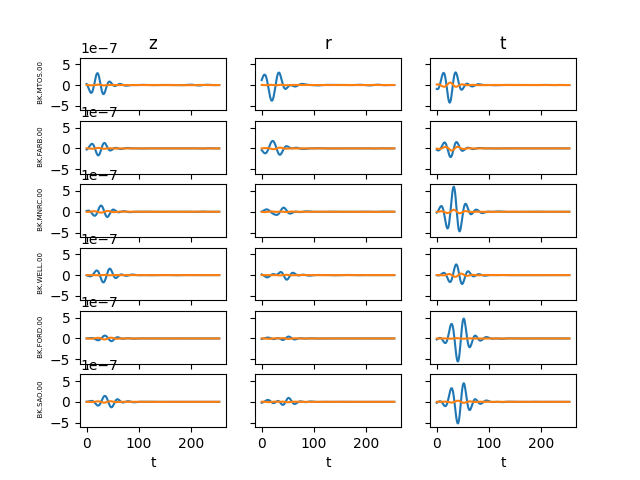
\includegraphics{dataSet1/plots/optimized0.png}
	\caption{target (blue) and average seismogram (orange) before optimization with DC mechanism}
	\label{convergenceDC1}
\end{figure}
\begin{figure}[H]
	\centering
	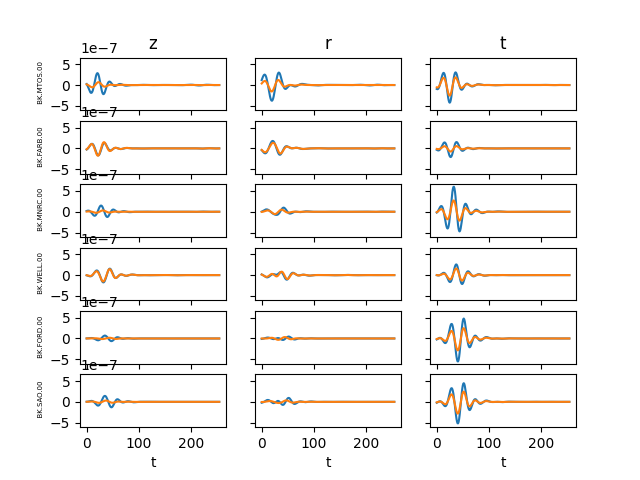
\includegraphics{dataSet1/plots/optimized3.png}
	\caption{target (blue) and optimized seismograms (orange) for iteration 4 of genetic algorithm with DC mechanism}
	\label{convergenceDC2}
\end{figure}
\begin{figure}[H]
	\centering
	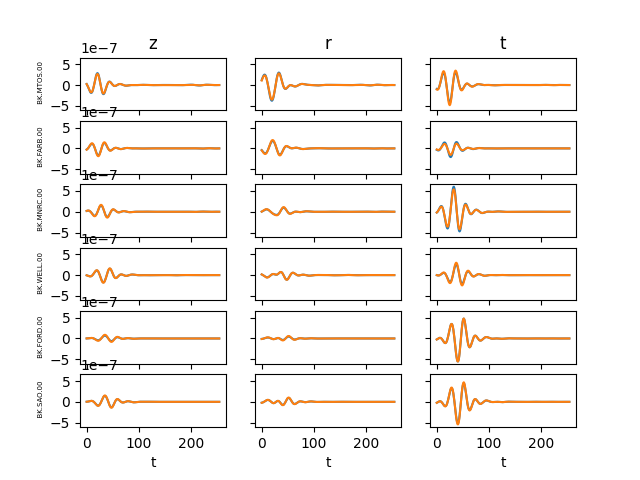
\includegraphics{dataSet1/plots/optimized49.png}
	\caption{Target (blue) and optimized seismograms (orange) for iteration 50 of genetic algorithm with DC mechanism}
	\label{convergenceDC3}
\end{figure}

Figures \ref{convergenceDC1}, \ref{convergenceDC2}, \ref{convergenceDC3} show that as the genetic algorithm iterates the optimized seismograms 
approach their target. This convergence can also be seen in figure \ref{scoresDC} which shows the score (similarity between target and optimized seismograms) increases as we iterate the program. This increase in score coencides with a decrease in deviation across the population of moment tensors as shown in figure \ref{MTDDC} and an increasing similarity between the average Moment tensor and the target moment tensor shown in figure \ref{MTSDC}. These features show the genetic algorithm converged to the correct solution. 
\begin{figure}[H]
	\centering
	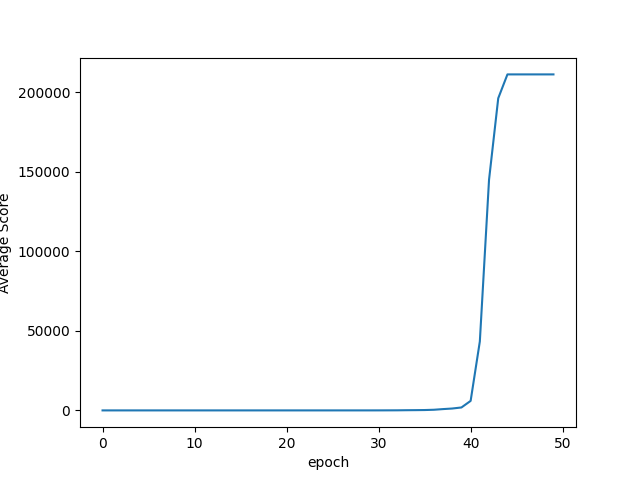
\includegraphics{dataSet1/scores.png}
	\caption{Average score of genetic population against number of generations (epochs) for DC target}
	\label{scoresDC}
\end{figure}

\begin{figure}[H]
	\centering
	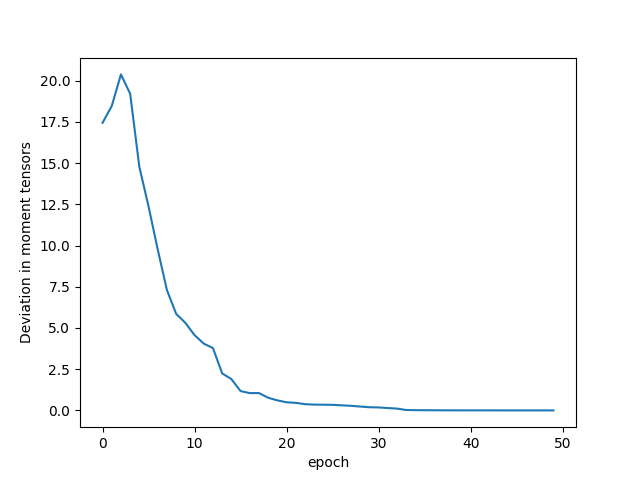
\includegraphics{dataSet1/MTDeviation.png}
	\caption{Deviation in moment tensor population against number of generations (epochs) for DC target}
	\label{MTDDC}
\end{figure}

\begin{figure}[H]
	\centering
	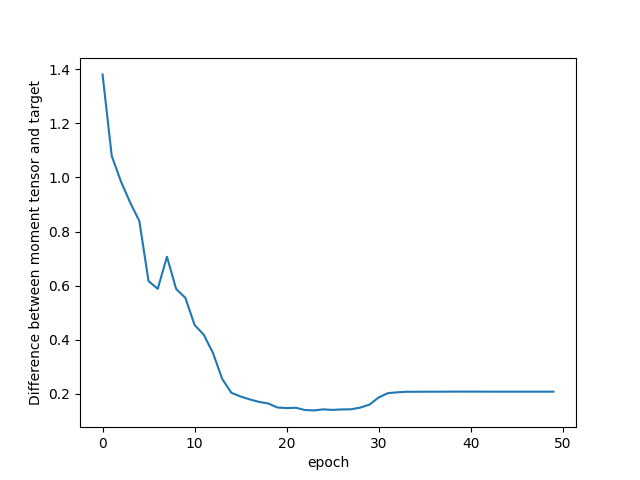
\includegraphics{dataSet1/MTsimilarity.png}
	\caption{Similarity between average moment tensor and number of generations (epochs) for DC target}
	\label{MTSDC}
\end{figure}


\subsection*{Isotropic result}
The target moment tensor is:
\begin{gather}
	\begin{pmatrix}
	0.5 & 0 & 0 \\
	0 & 0.5 & 0 \\
	0 & 0 & 0.5 
	\end{pmatrix}
\end{gather}
The program finds a moment tensor:
\begin{gather}
	\begin{pmatrix}
	0.20 & -0.00 & 0.00 \\
	-0.00 & 0.20 & -0.00 \\
	0.00 & -0.00 & -0.19 
	\end{pmatrix}
\end{gather}
This inversion is not very accurate, it has optimized all components with value 0 correctly, but gotten the wrong sign on $m_{zz}$ and the magnitudes for 
$m_{xx}$ and $m_{yy}$ are substantially different. It has found a pure CLVD moment tensor rather than an isotropic one! However, as seen in figure \ref{convergenceISO1}, \ref{convergenceISO2}, \ref{convergenceISO3} the optimized seismograms still converges to the target siesmograms. Figures \ref{scoresISO}, \ref{MTDISO}, \ref{MTSISO} show similar behviour to their DC counterparts confirming that the genetic algorithm did converge. However, the high gradient near the end of the simulation (40-50th iteration) in figure \ref{scoresISO} suggests the genetic algorithm could optimize further. This optimization would most likely be a refinement of the final moment tensor:
\begin{gather}
	\begin{pmatrix}
	0.20 & -0.00 & 0.00 \\
	-0.00 & 0.20 & -0.00 \\
	0.00 & -0.00 & -0.19 
	\end{pmatrix}
\end{gather}
and would still be substantially different from the target moment tensor due to the small deviation in the population of moment tensors on the final iteration (iteration 49) seen in figure \ref{MTDISO}. 

\begin{figure}[H]
	\centering
	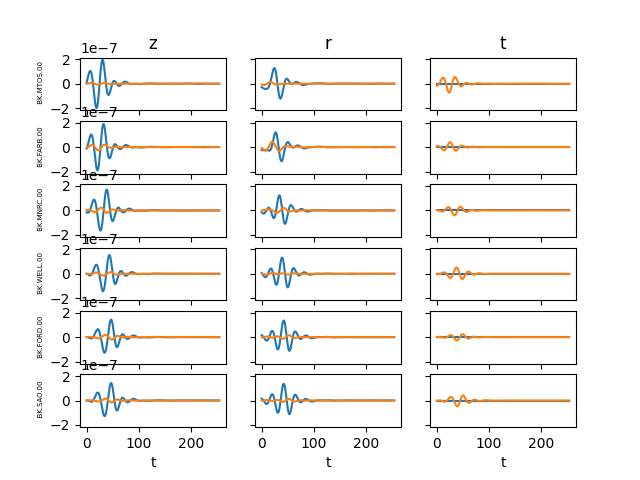
\includegraphics{dataSet2/plots/optimized0.png}
	\caption{target (blue) and average seismogram (orange) before optimization with ISO mechanism}
	\label{convergenceISO1}
\end{figure}
\begin{figure}[H]
	\centering
	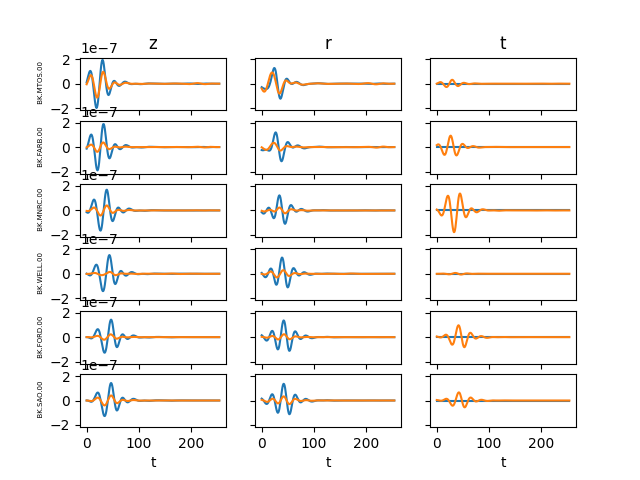
\includegraphics{dataSet2/plots/optimized3.png}
	\caption{target (blue) and optimized seismograms (orange) for iteration 4 of genetic algorithm with ISO mechanism}
	\label{convergenceISO2}
\end{figure}
\begin{figure}[H]
	\centering
	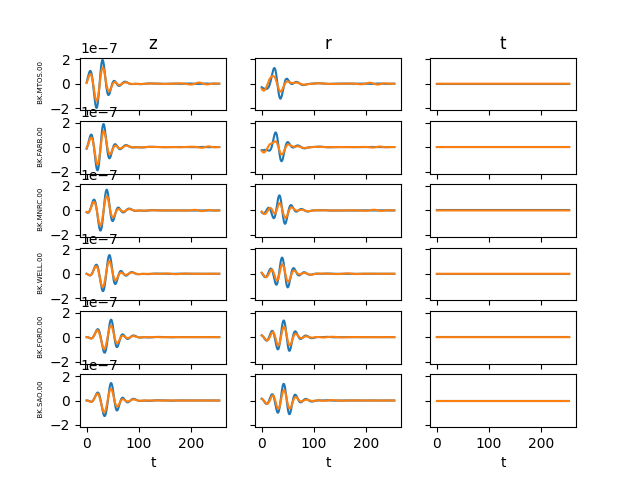
\includegraphics{dataSet2/plots/optimized49.png}
	\caption{Target (blue) and optimized seismograms (orange) for iteration 50 of genetic algorithm with ISO mechanism}
	\label{convergenceISO3}
\end{figure}

\begin{figure}[H]
	\centering
	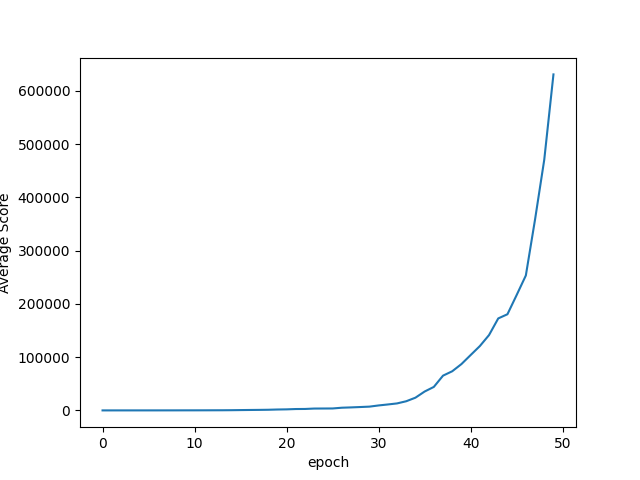
\includegraphics{dataSet2/scores.png}
	\caption{Average score of genetic population against number of generations (epochs) for ISO target}
	\label{scoresISO}
\end{figure}

\begin{figure}[H]
	\centering
	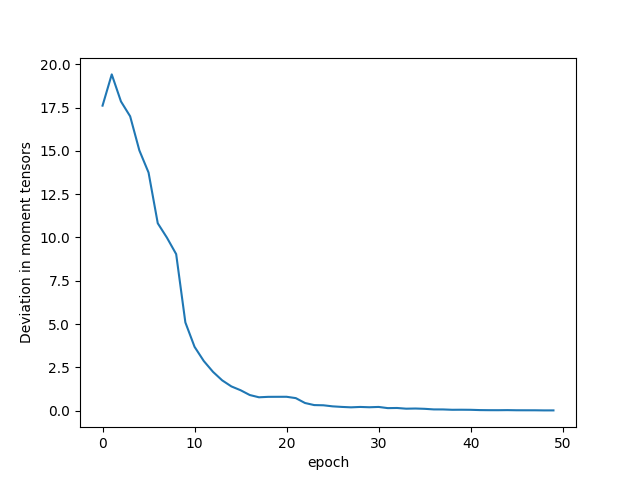
\includegraphics{dataSet2/MTDeviation.png}
	\caption{Deviation in moment tensor population against number of generations (epochs) for ISO target}
	\label{MTDISO}
\end{figure}

\begin{figure}[H]
	\centering
	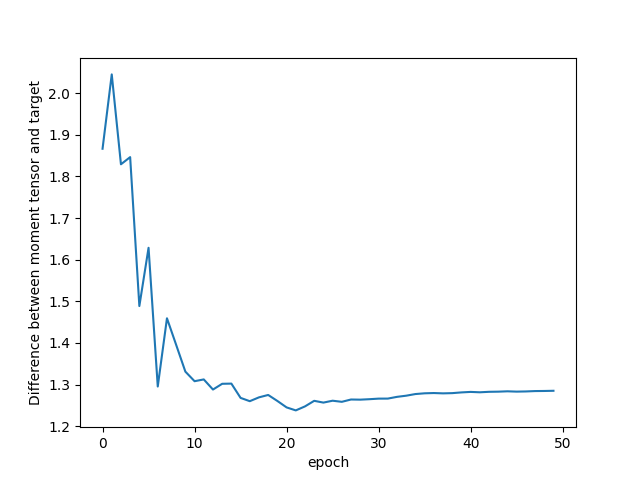
\includegraphics{dataSet2/MTsimilarity.png}
	\caption{Similarity between average moment tensor and number of generations (epochs) for ISO target}
	\label{MTSISO}
\end{figure}

\subsection*{CLVD results}
The target moment tensor is:
\begin{gather}
	\begin{pmatrix}
	0.25 & 0 & 0 \\
	0 & 0.25 & 0 \\
	0 & 0 & -0.5 
	\end{pmatrix}
\end{gather}
The program finds a moment tensor:
\begin{gather}
	\begin{pmatrix}
	-0.03 & -0.00 & 0.13 \\
	-0.01 & 0.06 & -0.04 \\
	0.12 & -0.04 & -0.14 
	\end{pmatrix}
\end{gather}
The optimized moment tensor is again substantually different from the target. The seismograms also did not converge correctly as seen in figure \ref{convergenceCLVD1}, \ref{convergenceCLVD2}, \ref{convergenceCLVD3}. The genetic algorithm did converge however, as shown by the decreasing deviation in the population of moment tensors (figure \ref{MTSCLVD}) and the flattening of the score in figure \ref{scoresCLVD}. Its just that this convergence was not to a good solution.

\begin{figure}[H]
	\centering
	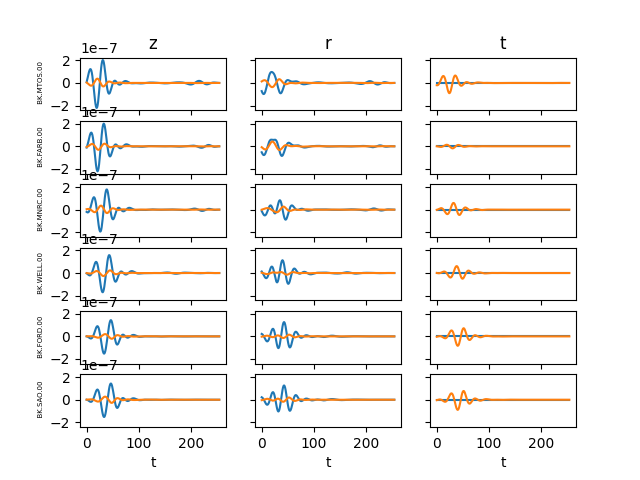
\includegraphics{dataSet3/plots/optimized0.png}
	\caption{target (blue) and average seismogram (orange) before optimization with CLVD mechanism}
	\label{convergenceCLVD1}
\end{figure}
\begin{figure}[H]
	\centering
	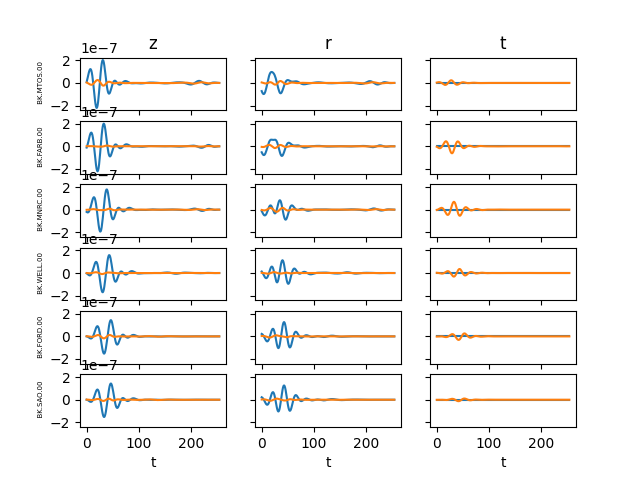
\includegraphics{dataSet3/plots/optimized3.png}
	\caption{target (blue) and optimized seismograms (orange) for iteration 4 of genetic algorithm with CLVD mechanism}
	\label{convergenceCLVD2}
\end{figure}
\begin{figure}[H]
	\centering
	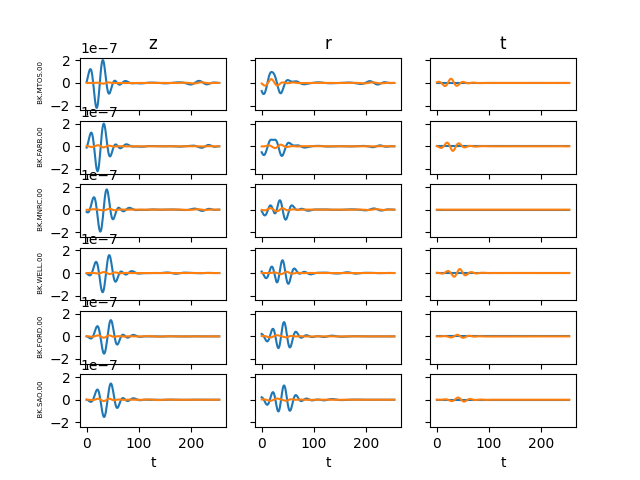
\includegraphics{dataSet3/plots/optimized49.png}
	\caption{Target (blue) and optimized seismograms (orange) for iteration 50 of genetic algorithm with CLVD mechanism}
	\label{convergenceCLVD3}
\end{figure}


\begin{figure}[H]
	\centering
	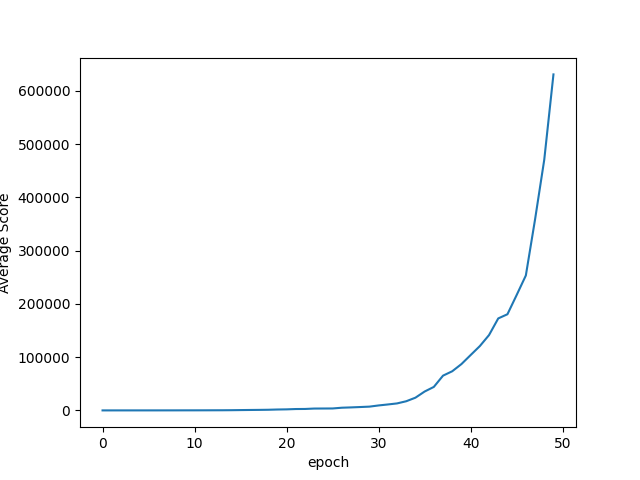
\includegraphics{dataSet2/scores.png}
	\caption{Average score of genetic population against number of generations (epochs) for CLVD target}
	\label{scoresCLVD}
\end{figure}

\begin{figure}[H]
	\centering
	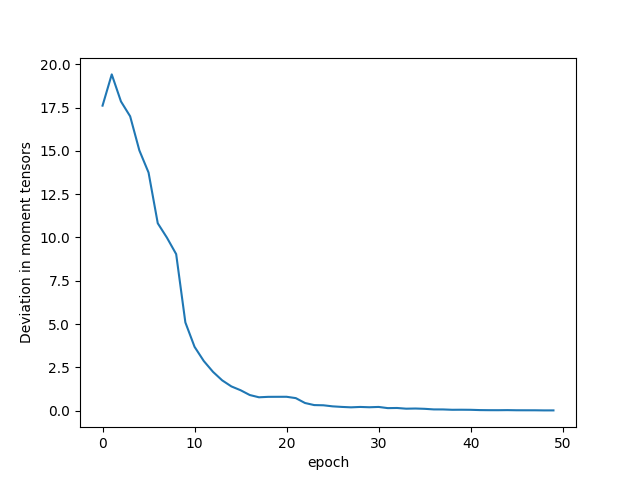
\includegraphics{dataSet2/MTDeviation.png}
	\caption{Deviation in moment tensor population against number of generations (epochs) for CLVD target}
	\label{MTDCLVD}
\end{figure}

\begin{figure}[H]
	\centering
	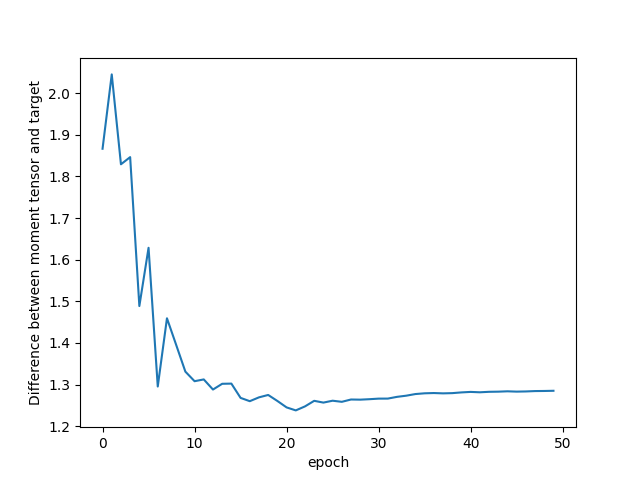
\includegraphics{dataSet2/MTsimilarity.png}
	\caption{Similarity between average moment tensor and number of generations (epochs) for CLVD target}
	\label{MTSCLVD}
\end{figure}

\subsection*{Summary of results}
The three components conveiently show the three different outcomes of running the genetic algorithm. The first outcome shown in the DC case 
is the algorithm converges to a highly optimized moment tensor that is the target moment tensor. The second outcome shown in the isotropic case is that the genetic algorithm converges to a high optimized moment tensor that is not the target. Finally, as shown in the isotropic case, the algorithm can converge to a poorly optimized moment tensor that does not match the target.
\newline
To remedy the second and third outcomes the genetic population could be increased. This increases computation time. The second outcome may also be a feature of the greens functions not giving suffecient information for a unique inversion which would not benifit from an increased genetic population.
\newline
The program is quite slow, even at the current settings which use a small genetic population of 100 and 50 generations it takes about 10 minutes to run. The program could be sped up by using a faster language such as goLang or C. 



\subsection*{Interesting Extensions}
An additional term can be added to the metric $g(\cdot, \cdot)$ that makes solutions unique in the population get higher scores and therefore more likely 
to breed and spread their influence onto the next generation. By adjusting this term and clustering moment tensor solutions rather than returning their 
average, multiple solutions that fit the situation well could be found. This may allow for multiple interpretations of the event which can be woven 
together with other observations to provide a more coherent picture of the situation. As far as I understand standard techniques do not accommodate this.


\section*{Appendix}
%% Here I want to have some definitions of metrics that I use

\subsection*{Definitions of metrics used}

\subsubsection*{Score or score metric}
The score metric is between two seismograms or sets of siemograms. For target seismogram d and another seismogram d', it is the sum $s(d,d') = \sum_{i} \sqrt{di**2}/\sqrt((di - di')**2)$. For a set of seismograms it is the sum over all $s(d,d')$ where d and d' are from the same station and are the same direction component.

\subsubsection*{Moment tensor deviation in a population}
A population is composed of a set of moment tensors. For element with indexes $i,j$ we find the maximum and minimum of $m_{i,j}$ where $m$ is a moment tensor in the population. The difference between the maximum and minimum is the deviation for index $i,j$. The deviation is then the sum of deviations for each indexes $i,j$.














\end{document}  

